\cotefile{79}
\scanpage{33}
\figure{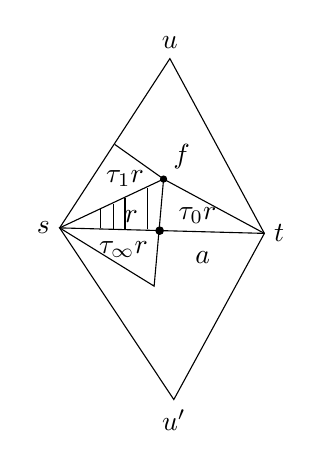
\begin{tikzpicture}[x=1cm,y=1cm,baseline]
\coordinate (s) at (0,0); \coordinate (t) at (2.6,-.07);
\coordinate (u) at (1.4,2.15); \coordinate (v) at (1.45,-2.18);
\coordinate (f) at (1.32,.62); \coordinate (a) at (1.27,-.035);
\draw (s)--(u)--(t)--(v)--cycle (s)--(t);
\draw (.70,1.06)--(f)--(t) (s)--(f)--(1.20,-.74)--cycle;
\foreach \x in {.52,.68,.83,1.12}{\draw (\x,-.013*\x)--(\x,.45*\x);}
\fill (f) circle (.046) (a) circle (.055);
\node[left] at (s){$s$}; \node[right] at (t){$t$};
\node[above] at (u){$u$}; \node[below] at (v){$u'$};
\node[above right] at (f){$f$}; \node[below right] at (1.60,-.18){$a$};
\node at (.83,.63){$\tau_1 r$}; \node at (1.75,.16){$\tau_0 r$};
\node at (.81,-.27){$\tau_\infty r$}; \node at (.91,.15){$r$};
\end{tikzpicture}}

Si $u'$ est le sommet de $SP_M$ tel que l'on ait
\[
\{s,t,u'\}\in SF_M \qquad \{s,t,u'\}\ne\{s,t,u\}\quad\text{i.e. }u'\ne u
\]
i.e.
\[
u'=(x-y)^{\bullet},\tag*{(81)}
\]
on aura
\[
\left\{\begin{aligned}
\tau_0^r(s,t,u)&=(t,s,u)\\
\tau_1^r(s,\deleted{\unsure{b}}t,u)&=(s,u,t)\\
\tau_\infty^r(s,t,u)&=(s,t,u')
\end{aligned}\right.
\qquad\text{\deleted{\illegible{1} est le \unsure{sommet}}}\tag*{(81)}
\]
donc $\tau_0^r,\tau_1^r,\tau_\infty^r$ sont induits respectivement par les automorphismes \inserted{antisymplectiques} de $M$, \unsure{qui|que} \deleted{\unsure{transf}}\deleted{\unsure{transforment}} sont caractérisés par
\[
\left\{\begin{aligned}
\tau_0^r\;&\left\{\begin{aligned}x&\mapsto y\\y&\unsure{\vdash\!\dashv|\mapsto}x\\z&\mapsto z\end{aligned}\right.
&&\text{matrice }\begin{pmatrix}0&1\\1&0\end{pmatrix}=r_0^{\deleted{\unsure{r}}}\\[3pt]
\tau_1^r\;&\left\{\begin{aligned}x&\mapsto x\\y&\mapsto \deleted{\unsure{y}}z\\z&\unsure{\vdash|\mapsto}y\end{aligned}\right.
&&\text{matrice }\begin{pmatrix}1&-1\\0&-1\end{pmatrix}=-r_1\\[3pt]
\tau_\infty^r\;&\left\{\begin{aligned}x&\mapsto x\\y&\mapsto-y\\z&\mapsto y-x\end{aligned}\right.
&&\text{matrice }\begin{pmatrix}1&0\\0&-1\end{pmatrix}=-r_\infty
\end{aligned}\right.\tag*{(82)}
\]
les automorphismes correspondants de $M$, et leurs matrices p.r. à la base $(x,y)$ de $M$, sont déterminés modulo signe par le choix du repère $r$ (et $=$, pour ce qui est des matrices, indépendamment du choix du repère). On trouve
\[
\left\{\begin{aligned}
\rho_0^r&\overset{\mathrm{déf}}{=}\tau_\infty^r\tau_1^r\mapsto\begin{pmatrix}1&-1\\0&1\end{pmatrix}=\lambda_0\\
\rho_1^r&\overset{\mathrm{déf}}{=}\tau_0^r\tau_\infty^r\mapsto\begin{pmatrix}0&-1\\1&0\end{pmatrix}=-\lambda_1\\
\rho_\infty^r&\overset{\mathrm{déf}}{=}\tau_1^r\tau_0^r\mapsto\begin{pmatrix}-1&1\\-1&0\end{pmatrix}=-\lambda_\infty
\end{aligned}\right.,\tag*{(83)}
\]
i.e. à des différences de signe près (qui du reste
% archive sheet number: 32
\scanpage{34}
\mspage{16}
point de vue actuel sont sans importance, puisqu'on travaille dans $\mathrm{Sl}(2,\Lambda)'$) on tombe pile sur les formules du formulaire 1981, qui avaient été obtenues par voie topologico-transcendante (classique) relativement délicate. Cel\unsure{a} confirme que ledit formulaire (où \inserted{le couple} des matrices $\rho=\lambda_\infty^{-1}$ et $\sigma=\lambda_1$ choisies comme générateurs de $\mathrm{Sl}(2,\mathbb Z)$, \deleted{par}
\[
\mathrm{Sl}(2,\mathbb Z)=\{\rho,\sigma\mid\rho^3=\sigma^2=\rho^{-3}\}\tag*{(84)}
\]
\deleted{sont bel et bien}\inserted{n'était défini, \deleted{\unsure{via|par|que par}}} ses propriétés intrinsèques remarquables, qu'à conjugaison près par un élément de $\mathrm{Gl}(2,\mathbb Z)/\{\pm1\}\simeq\mathrm{GP}(1,\mathbb Z)$) \deleted{\unsure{est}}était vraiment ``le plus naturel possible''.

\uline{NB} Si on regarde les homomorphismes
\[
\Pi_{0,3}=\{\rho_0,\rho_1,\rho_\infty\mid\rho_\infty\rho_1\rho_0=1\}\xrightarrow{\varphi^\bullet}\mathrm{Sl}(2,\mathbb Z)\tag*{(85)}
\]
qui relèvent l'homomorphisme précédent à valeurs dans $\mathrm{Sl}(2,\mathbb Z)'$
\[
\rho_0\mapsto\lambda_0^\bullet,\ \rho_1\mapsto\lambda_1^\bullet,\ \rho_\infty\mapsto\lambda_\infty^\bullet,\tag*{(*)}
\]
ou les homomorphismes
\[
\Pi_{0,3}^{\tau}=\{\tau_0,\tau_1,\tau_\infty\mid\tau_{\unsure{0|\infty}}^2=\tau_1^2=\tau_\infty^2\}\xrightarrow{\varphi}\mathrm{Gl}(2,\mathbb Z)\tag*{(86)}
\]
qui relèvent l'hom précédent dans $\mathrm{Gl}(2,\mathbb Z)'\simeq\unsure{\mathrm{GP}(1,\mathbb Z)}$
\[
\tau_0\mapsto r_0^\bullet,\ \tau_1\mapsto r_1^\bullet,\ \tau_\infty\mapsto r_\infty^\bullet\tag*{(**)}
\]
(en partant du fait que pour $(*)$ et $(**)$ il y a des choix canoniques concordants, sans \deleted{\unsure{fixation}}\inserted{\unsure{ambi-|aucune}}
% archive sheet number: 33
\scanpage{35}
d'ambiguïté de signe), on trouve que pour un tel choix, disons
\[
\deleted{\unsure{\rho_0}}\quad\rho_0\mapsto\lambda_0,\quad\rho_1\mapsto\lambda_1,\quad\rho_\infty\mapsto\lambda_\infty\tag*{(87)}
\]
ou
\[
\tau_0\mapsto r_0,\quad\tau_1\unsure{\longrightarrow|\text{---}}r_1,\quad\tau_\infty\mapsto r_\infty,\tag*{(87 bis)}
\]
les autres choix possibles s'obtiennent en faisant des changements de signe sur les valeurs des images des $\rho_i$ resp. des $\tau_i$, avec comme seule contrainte que dans le cas des $\rho_i$, le nb de signes $-$ soit pair (donc égal à 2, \deleted{\unsure{3}}s'il y a effectivement modification). D'ailleurs, une fois le choix fait pour les $\rho_i$, si on veut que $\varphi^\circ$ soit induit par $\varphi$, cela impose le choix des images des $\tau_i$, au changement de signes \uline{simultané} près. Ceci vu, on tient à ce que l'image de $\rho_0$ soit \inserted{une matrice} unipotente, ce qui élimine l'ambiguïté de signe pour $\lambda_0$. \deleted{Cela} Il reste donc comme seule autre possibilité, en plus de (87), la possibilité
\[
\rho_0\mapsto\lambda_0,\ \rho_1\mapsto-\lambda_1,\ \rho_\infty\mapsto-\lambda_\infty\tag*{(88)}
\]
qui est celle qui s'est présentée dans (83). Elle se distingue du choix (87) par le fait que
\[
(-\lambda_\infty)^3=-(\lambda_\infty)^3=1,\quad\text{mais }\ (\lambda_\infty)^3=-1
\]
i.e. $-\lambda_\infty$ est d'ordre 3, tandis que $\lambda_\infty$ est d'ordre 6. Suivant le contexte, l'un ou l'autre des deux choix
% archive sheet number: 34
\scanpage{36}
\mspage{17}
peut être préférable -- l'an dernier j'ai choisi délibérément l'image de $\deleted{\unsure{\mathrm R}}\rho_\infty$ comme \inserted{$\lambda_\infty=$} $\rho^{-1}$ et non $-\rho^{-1}$, pour avoir un élément d'ordre 6, ``moins spécial'' donc que $-\lambda_\infty$ qui est d'ordre 3.

Relativement au choix (87)\inserted{$=(69)$} pour les $\rho_i$, on a le choix correspondant \inserted{$(87\ \mathrm{bis})=$}(72) pour les $\tau_i$, qui semble plus satisfaisant que l'autre choix possible
\[
\tau_i\mapsto-r_i,
\]
qui introduit plus de signes dans les expressions matricielles. Relativement au choix $(88)=(83)$, \unsure{le} choix \deleted{\unsure{cor}} compatible pour les $\tau_i$ est donné par (82), \deleted{\unsure{qu'on p|qui}}
\[
\tau_0\mapsto r_0,\quad\tau_1\longrightarrow-\unsure{\tau_1|r_1},\quad\tau_\infty\mapsto-r_\infty
\]
qu'on pourrait aussi remplacer par
\[
\tau_0\mapsto\unsure{-|\deleted{-}}r_0,\quad\tau_1\longrightarrow r_1,\quad\tau_\infty\mapsto r_\infty,
\]
mais qui n'a pas une signification géométrique aussi simple, en termes d'une action sur un $(x,y,z)\in B\deleted{\unsure{_{\varphi}}}(M)$\,; comme étant resp. la transposition de $x$ et $y$, de $y$ et $z$, ou la symétrie p.r. à l'axe des $x$

\deleted{(symétries p.r. à la diagonale principale, la diagonale non principale, et l'axe des $x$ dans le syst. de coordonnées défini par la base $(x,y)$ de $M$ \ldots)}
% archive sheet number: 35
\scanpage{37}
La construction du \S~I nous fournit donc des éléments remarquables
\[
\left\{\begin{aligned}
r_0,r_1,r_\infty&\in\mathrm{Gl}(2,\mathbb Z)\\
\lambda_0,\lambda_1,\lambda_\infty&\in\mathrm{Sl}(\unsure{1|2},\unsure{2|\mathbb Z})
\end{aligned}\right.
\]
satisfaisant les relations remarquables
\[
\left\{\begin{aligned}
&r_0^2=r_1^2=r_\infty^2=1\\
&\lambda_0=r_\infty r_1,\ \lambda_1=r_0r_\infty,\ \lambda_\infty=r_1r_0
&&\text{d'où }\lambda_\infty\lambda_1\lambda_0=1\\
&\lambda_\infty^{\deleted{6}3}=\lambda_1^2=\omega\ \text{(matrice $-1$)},&&\text{d'où }\lambda_\infty^6=\lambda_1^{\unsure{4|1}}=1\,;
\end{aligned}\right.
\]
sans impliquer pourtant que les hom correspondants
\[
\left\{\begin{aligned}
G^\circ_{\deleted{\unsure{3}}\infty,3}&\longrightarrow\mathrm{Sl}(2,\mathbb Z)'\\
G_{\infty,3}&\longrightarrow\mathrm{Gl}(2,\mathbb Z)'
\end{aligned}\right.
\]
sont des isomorphismes, i.e. sans impliquer
\[
\left\{\begin{aligned}
\mathrm{Sl}(2,\mathbb Z)'&\simeq\{\dot{\lambda}_1,\dot{\lambda}_\infty\mid\dot{\lambda}_1^2=\dot{\lambda}_\infty^3=1\}\\
\mathrm{Gl}(2,\mathbb Z)'&\simeq\{\dot{r}_0,\dot{r}_1,\dot{r}_\infty\mid
\dot{r}_0^2=\dot{r}_1^{\unsure{7|2}}=\dot{r}_\infty^2=(r_0r_\infty)^2=(r_1r_0)^3=1\}
\end{aligned}\right.
\]
Le fait qu'il en est bien ainsi \deleted{\unsure{rés}}\unsure{est une} identité remarquable, dont je ne connais pas de démonstration par voie purement algébrique. Je peux l'énoncer en disant que la structure 2-polyédrale triangulée orientée régulière, \deleted{déf} $SP_{\deleted{\unsure{\Lambda}}M\unsure{=}}$, définie par un $\mathbb Z$-module \deleted{\unsure{de}} libre de rg 2 muni d'une base symplectique, est \uline{universelle}, en ce sens
% archive sheet number: 36
\scanpage{38}
\mspage{18}
que si on choisit un repère direct $r_0$ \deleted{\unsure{$\in SR$}} de $\deleted{\unsure{B}}SP_M$ -- ce qui revient à se donner une base symplectique $M\simeq\mathbb Z^2$ --, alors pour toute structure 2-polyédrale triangulée orientée $P$ et \unsure{tout} repère $r$ de $P$, il existe un homomorphisme et un seul
\[
\left\{\begin{aligned}
SF_M&\longrightarrow P&&\text{tel que}\\
r_0&\longmapsto r&&.
\end{aligned}\right.
\]

\(\overline{\underline{\mathrm{III}}}\)

Quand on se donne un module libre \inserted{$M$} de rang 2 sur un anneau $\Lambda$ \inserted{\deleted{\unsure{``ab}} ``absolu'' i.e.} isomorphe à \deleted{\unsure{un}} $\mathbb Z$ ou à un $\mathbb Z/n\mathbb Z$ (où on suppose néanmoins $n\geqslant3$), sans se donner de structure symplectique \inserted{$e_M$} ou semi-symplectique $\{\pm e_M\}$\,; on peut néanmoins lui associer encore un 2-polyèdre \inserted{triangulé} régulier, \deleted{de la} \inserted{dont \unsure{le|l'} $\pi_0$ est} paramétré par l'ensemble quotient
\[
(\mathrm{dét}\,M)^*/\pm1\simeq\mathrm{Ssympl}(M).\tag*{(89)}
\]
formé des structures $\tfrac12$ symplectiques sur $M$,
\margin{On a donc changé la notation p.r. à (23), qui finalement n'introduit pas ``le bon'' objet\ldots}
% slanted
en prenant le \inserted{polyèdre $P_M$} somme directe des 2-polyèdres réguliers triangulés (\uline{non} \uline{orientés}) associés aux diverses structures semisymplectiques sur $M$.

Notons que pour
\[
\mu\in(\mathrm{det}\,M)^*/\{\pm1\}\tag*{(90)}
\]
% archive sheet number: 37
\scanpage{39}
i.e.
\[
\mu\subset(\mathrm{dét}\,M)^*\qquad\mu=-\mu,\quad\mathrm{card}\,\mu=2,
\]
le \deleted{\unsure{l'ens}} polyèdre régulier $SF_{M,\mu}$ admet un iso. can.
\[
\underline{\mathrm{Or}}(SF_{M,\mu})\simeq\mu\tag*{(91)}
\]
Pour $\Lambda=\mathbb Z$, $(\mathrm{det}\,M)^*$ est déjà réduit à deux éléments, et \deleted{\unsure{$P$}} $P_M$ est un 2-polyèdre régulier connexe, dont l'ens des orientations est en bijection can. avec $\mu=(\mathrm{det}\,M)^*$. Pour $\Lambda=\mathbb Z/n\mathbb Z$, avec $n\geqslant3$, alors $(\mathrm{det}\,M)^*/\{\pm1\}$ est de cardinal $\varphi(n)/2$, donc $P_M$ a $\varphi(n)/2$ composantes connexes. Il est connexe sss $\varphi(n)\ne2=1$, i.e.
\[
P_M\ \text{connexe}\iff\varphi(n)=2\iff n\in\{3,4,6\},\tag*{(92)}
\]
le premier cas où $P_M$ est disconnexe étant relatif à la valeur $n=5$, où on trouve pour $P_M$ un ``biicosaèdre''. Il faudrait revenir sur ce cas par la suite (ainsi que \deleted{sur tous} \inserted{sur chacun} des cas $n\in\{3,4,5,6\}$). Pour le moment, je voudrais, dans le cas $\Lambda$ fini i.e. $\Lambda\simeq\mathbb Z/n\mathbb Z$, et dans le cas $P_M$ disconnexe i.e. $n=5$ ou $n\geqslant7$, dégager des éléments de structure supplé%
% archive sheet number: 38
\scanpage{40}%
\mspage{19}%
mentaires de $P_M$, qui permettraient peut-être d'identifier $\mathrm{Gl}_\Lambda(M)'=\mathrm{Gl}_\Lambda(M)/\{\pm\mathrm{id}_M\}$ au groupe des automorphismes de la structure renforcée.

Je désigne par
\[
\dot g\mapsto T_{\dot g}:\quad\mathrm{Gl}_\Lambda(M)'\longrightarrow\mathrm{Aut}(P_M)\tag*{(93)}
\]
l'opération naturelle de $\mathrm{Gl}_\Lambda(M)'$ sur $P_M$, et je \deleted{\unsure{considè|considère}} pose
\[
Z'_\Lambda=\Lambda^*/\{\pm1_\Lambda\}\subset\mathrm{Gl}_\Lambda(M)'\tag*{(94)}
\]
c'est un sous-groupe central, égal au centre de $\mathrm{Gl}_\Lambda(M)'$ sauf erreur,

je considère comme première structure suppl. sur $P_M$ la restriction de l'opération (93) de $\mathrm{Gl}_\Lambda(M)'$ sur $P_M$ au ss-groupe $Z'_\Lambda$
\[
\begin{aligned}
Z'_\Lambda&\longrightarrow\unsure{\mathrm{Aut}|\mathrm{Aut}_\Lambda}(P_M)\\
\dot\lambda&\longmapsto T_{\dot\lambda}
\end{aligned}.\tag*{(95)}
\]
D'autre part, \deleted{je} rappelons nous de la bijection canonique
\[
\pi_0(P_M)\simeq(\mathrm{det}\,M)^*/\{\pm1_\Lambda\},\tag*{(96)}
\]
qui donne une opération
\[
\dot\lambda\longmapsto\bigl(\dot\lambda_\pi:i\mapsto\dot\lambda.i\bigr)
\qquad Z'_M\longrightarrow\unsure{\mathfrak S|\mathscr S}_{\pi_0(P_M)}\tag*{(97)}
\]
de $Z'_\Lambda$ sur $\pi_0(P_M)$, faisant de $\pi_0(P_M)$ un \uline{torseur} sous $Z'_\Lambda$. Pour $\dot g\in\mathrm{Gl}_\Lambda(M)'$, $i\in\pi_0(P_M)$,
% archive sheet number: 39
\scanpage{41}
on a alors
\[
T_{\dot g}i=(\mathrm{det}(\dot g))^\bullet.i\tag*{(98)}
\]
ce qui relie (93) et (97), et caractérise en fait (97) en termes de (93). Pour $\dot g$ de la forme $\dot\lambda$, avec $\dot\lambda\in Z'_{\unsure{\Lambda|M}}$, on trouve donc
\[
T_{\dot\lambda}i=\dot\lambda^2.i\qquad\dot\lambda\in Z'_\Lambda,\quad i\in\pi_0(P_M),\tag*{(99)}
\]
formule qui relie les deux éléments de structure (95) et (97).

Enfin, rappelons nous des bijections canoniques
\[
\deleted{\unsure{P}}S_{M,i}\simeq M^*\qquad i\in\pi_0(P_M),\tag*{(100)}
\]
où $\deleted{\unsure{P}}S_{M,i}$ désigne la \inserted{l'ens des sommets de la} composante connexe $P_{M,i}$ de $P_M$ d'indice $i$ -- ces bijections canoniques définissent \deleted{\unsure{une}},
\[
\left\{\begin{aligned}
&\text{un syst. transitif de bijections canoniques}\\
&\mathrm{tr}_{\unsure{s|S}\,ji}:S_{M,i}\overset{\sim}{\text{---}} S_{M,j}
\qquad(i,j\in\pi_0(P_M)).
\end{aligned}\right.\tag*{(101)}
\]
Appelons \uline{automorphisme strict} de $P_M$ tout automorphisme \deleted{\unsure{qui conserve}}\inserted{du polyèdre qui} respecte les trois structures supplémentaires (95) (97) (101).
\margin{On verra par la suite que les \unsure{deux} structures (95) (97) sont inutiles}
% slanted
Désignons \deleted{alors \unsure{avec}} \inserted{par $\mathrm{Autstr}$}$(P_M)$
% archive sheet number: 40
\scanpage{42}
Pour la surjectivité, il suffit de prouver celle de
\[
\mathrm{Gl}'_\Lambda(M)^\pm\longrightarrow\mathrm{Autstr}_{\deleted{\unsure{1}}}^{\unsure{\circ|0}}(\deleted{\unsure{M}}P_M).
\]
Soit donc $u\in\mathrm{Autstr}^{\circ}(P_M)$, choisissons un \deleted{\unsure{$e$}} $i\in\pi_0(P_M)\simeq(\mathrm{det}\,M)^*/\pm1$, $i=\{\pm e_M\}$, et considérons l'autom de $P_{M,i}$ induit par $u$. Par ce qu'on a vu, $\exists\unsure{1|\vert|!}\,\dot g\in\mathrm{Gl}'_\Lambda(M)^\pm$, tel que $T_{\dot g}\mid P_{M,i}=u\mid P_{M,i}$. On est donc ramené au cas où \deleted{\unsure{$g$}} $u\mid P_{M,i}=\mathrm{id}_{P_{M,i}}$, et à prouver qu'alors $u=\mathrm{id}_{P_M}$, ou ce qui revient au $=$, que $u$ induit l'identité sur \deleted{\unsure{$SP$}} l'ens des sommets $S_{P_M}$ de $P_M$. Mais cela provient du fait que $u$ induit l'identité sur $\deleted{\unsure{S_{P_{M,i}}=|S_{P_{M,i}}}}S_{M,i}$, et qu'il respecte la \deleted{\unsure{syst}} structure (101), cqfd.

\uline{Remarque} Dans cette démonstration, on n'a pas utilisé, dans la définition de $\mathrm{Autstr}(P_M)$, que les $u$ envisagés respectent la structure (95), mais seulement (97) et (101). \margin{en fait, $=$ (97) est \uline{inutile}, cf \S~V, p.~\unsure{44$^\circ$|44$^o$}}
% slanted
Donc on voit a posteriori qu'un tel autom.
% archive sheet number: 41
\scanpage{43}
\mspage{20}
le groupe qu'ils forment, et par $\mathrm{Autstr}^{\unsure{\circ|0}}(P_M)$ le sous-groupe formé des $u$ qui induisent l'identité sur $\pi_0(P_M)$. On trouve donc une suite exacte canonique
\[
1\longrightarrow\mathrm{Autstr}^\circ(P_M)\longrightarrow\mathrm{Autstr}(P_M)\xrightarrow{\delta} Z'_\Lambda\longrightarrow1,\tag*{(102)}
\]
où l'hom $\delta$ est défini via l'opération d'un $\deleted{\unsure{P_M\ \mathrm{sur}}}u\in\mathrm{Autstr}(P_M)$ sur $\pi_0(P_M)$, qui doit être de la forme $i\mapsto\deleted{\unsure{\lambda_\delta}}\delta(u).i$, pour un $\delta(u)\in Z'_\Lambda$ bien déterminé (puisque $u$ \deleted{conserve}\inserted{respecte} la structure (97)). Considérons maintenant l'hom canonique de suites exactes, \deleted{déduit} de la suite exacte
\[
1\longrightarrow\mathrm{Gl}'_\Lambda(M)^\pm\longrightarrow\mathrm{Gl}_\Lambda(M)'\longrightarrow\Lambda^*/\pm1_\Lambda\unsure{\text{---}|\longrightarrow}1\tag*{(103)}
\]
dans (102), induite par $\dot g\mapsto T_{\dot g}$\,:

\diagram{\small\[\begin{tikzcd}[ampersand replacement=\&,column sep=small,row sep=large]
1\arrow[r]\&\mathrm{Gl}'_\Lambda(M)^\pm\arrow[r]\arrow[d]\&\mathrm{Gl}_\Lambda(M)'\arrow[r]\arrow[d,"{\dot g\mapsto T_{\dot g}}"]\&\Lambda^*/\{\pm1_\Lambda\}\arrow[r]\arrow[d,"1"]\&1\\
1\arrow[r]\&\mathrm{Autstr}^\circ(P_M)\arrow[r]\&\mathrm{Autstr}(P_M)\arrow[r]\&Z'_\Lambda\arrow[r]\&1
\end{tikzcd}\tag*{(104)}\]}

\noindent\begin{tabular}{|p{.91\linewidth}}
\uline{Théorème}\quad L'hom de suites exactes (104) est un iso.
\end{tabular}

L'injectivité de $\dot g\mapsto T_{\dot g}$ est immédiate, elle provient de l'injectivité \deleted{de} $\mathrm{Gl}'_\Lambda(M)^\pm\longrightarrow\mathrm{Aut}(SP_{(M,e_M)})$, déjà vue (cette dernière flèche étant en fait bijective).
% archive sheet number: 42
\scanpage{44}
\mspage{21}
respecte également la structure (95). Il serait bon d'en comprendre la raison a priori.

\deleted{Pour ceci, je note que l'action d'un autom. \deleted{de} $u$ de $P_M$ est connue, quand on la connaît sur l'ens des sommets $S_{P_M}$, puisque les \deleted{\unsure{$S$}} ens des arêtes et \deleted{\unsure{$F$}} \unsure{ens} des faces s'identifient à des ens. de parties (à deux \deleted{\unsure{ou}} et à trois éléments respectivement) de $S_{P_M}$. D'autre part, un autom. \inserted{\unsure{$u$|``}}qui respecte la structure (101) est connu quand on connaît son action sur $\pi_0(P_M)$, \uline{et} sur \uline{un} $S_{M,i}$. Quand $u$ respecte \inserted{aussi} la structure (97), l'action de $u$ sur $\pi_0(P_M)$ se décrit via $\delta(u)\in Z'_\Lambda$. Lorsque $u$ est de la forme $T_{\dot\lambda}$, $\dot\lambda\in Z'_\Lambda$, on a $\delta(u)=\dot\lambda^2$, i.e l'action de $T_{\dot\lambda}$ sur $\pi_0(P_M)$ est déterminée par la structure (97).}
\margin{\uline{NB} On a en vertu des structures (97) (101) $S_{P_M}\simeq I_M\times\pi_0(P_M)$, où $I_M$ est ``la val. commune'' des $S_{P_M,i}$, identifiés via les \unsure{tr} de (101).}
% slanted

Récapitulons le type d'objet structuré qui est pour nous $P_M$. \deleted{Il}\unsure{Il|On} peut \unsure{se|le} décrire par les données
\[
\left\{\begin{aligned}
&\deleted{I}S\ \text{un ens }\deleted{\unsure{\ne\varnothing|\text{fini}}}\inserted{\text{(de cardinal $\geqslant3$)}}\
\text{(la ``valeur commune'' des }\deleted{\unsure{S_{M,i}}}S_{P_M,i},\ \text{pour }i\in\pi_0(P_M)),\\
&\pi\ \text{un }Z'_\Lambda\text{-torseur}\qquad(Z'_\Lambda=\Lambda^*/\{\pm1_\Lambda\})\\
&\pi\xrightarrow{\Sigma}\unsure{\mathfrak P|\mathcal P}(\mathfrak P_3(\deleted{I}S))\quad\text{une application}
\end{aligned}\right.\tag*{(105)}
\]
\margin{en fait $\mathrm{card}\,S\geqslant4$}
% slanted
satisfaisant les conditions nécessaires suivantes\,:
\[
\left\{\begin{aligned}
&\text{\textcircled{a}}\quad\forall\,i\in\pi,\quad \Sigma(i)\in\mathfrak P(\mathfrak P_3(\unsure{I|S|\mathbb S}))\ \text{est une structure}\\
&\hspace{4em}\text{de 2-polyèdre triangulé }\inserted{\text{connexe}}\ \text{sur }\deleted{I}S,\ \deleted{\text{soit}}\\
&\deleted{\text{b) Les }u\in\mathfrak S_I\ \text{qui sont des autom.}}
\end{aligned}\right.\tag*{(106)}
\]
% archive sheet number: 43
\scanpage{45}
\deleted{(106) b) Soit $G_i\overset{\unsure{\mathrm{déf}}}{=}\{u\in\unsure{\mathfrak S|\mathscr S}_I\mid u$ est un $\Sigma(i)$-autom. de $S$, $\forall i\in\pi\}$ \deleted{alors}\inserted{de $i$ ?} \inserted{$\mathrm{Aut}(S,\Sigma(i))$, alors $G_i$ est indépendant}}

\[
\text{\textcircled{b}}\quad \forall i\in\pi,\quad\text{soit }\ G_i=\mathrm{Aut}(S,\Sigma(i))\inserted{\subset\mathfrak S_S},\quad\text{alors}\tag*{(107)}
\]
$G_i$ est indépendant de $i\in\pi$, \inserted{soit $G$} (il y a vraiment du mérite\,\unsure{!|?}, d'autant plus que l'on a c) ci-dessous)

\margin{On a aussi que $G_i^+$ \deleted{\unsure{$g$}} est indépendant de $i$, et que $G^{\deleted{\unsure{+}}}$ (resp. $G^+$) est simpl$^{\mathrm t}$. transitif sur l'ens des repères (resp des repères directs) de $\Sigma(i)$, i.e. que $(S,\Sigma(i))$ est un ``2-polyèdre \uline{régulier} (aux deux sens).}
% slanted
\margin{\uline{Question} Y a-t-il d'autres structures triangulées \deleted{rég.} sur $S$, isomorphes aux structures envisagées, et qui ont les $=^{\mathrm s}$ groupes d'autom $G,G^+$ ?}
% slanted
\[
\text{\textcircled{c}}\quad \pi\unsure{\overset{\Sigma}{\longleftrightarrow}|\xrightarrow{\Sigma}}\unsure{\mathfrak P|\mathcal P}(\mathfrak P_3(S))\quad\text{est \uline{injectif}}\tag*{(108)}
\]
i.e. $i\unsure{=|\ne}j\implies\Sigma(i)\unsure{=|\ne}\Sigma(j)$, plus précisément,
\[
i\ne j\implies\left\{\begin{aligned}
A_{\Sigma(i)}\cap A_{\Sigma(j)}&=\varnothing\\
F_{\Sigma(i)}\cap F_{\Sigma(j)}&=\varnothing
\end{aligned}\right.
\]
où $A_{\Sigma(i)},F_{\Sigma(i)}\inserted{=\Sigma(i)}$ est l'ens des arêtes resp. des faces pour \deleted{$\Sigma(i)$} la structure $\Sigma(i)$.

Dans les propriétés a) b) c) ci-dessus, la structure de torseur sur $\pi$ n'est pas intervenue encore. Introduisant cette structure, on trouve, en désignant par $\mathcal A$ le groupe des autom de la structure (105)
\[
1\longrightarrow G\longrightarrow\mathcal A
\xrightarrow[\substack{\text{via action}\\\text{de }\mathcal A\text{ sur}}]{\delta}Z'_\Lambda
\]
et on a
\[
\begin{aligned}
&\text{\textcircled{d}}\quad\text{L'hom }\mathcal A\longrightarrow Z'_\Lambda=(\mathbb Z/n\mathbb Z)^*/\{\pm1\}\\
&\qquad\text{précédent est surjectif.}
\end{aligned}\tag*{(109)}
\]
On a
\[
\begin{aligned}
&\text{\textcircled{e}}\quad\forall\dot\lambda\in Z'_\Lambda,\quad\exists\unsure{1|\vert|!}\ T_{\dot\lambda}\in\mathfrak S_S,\quad\text{tel que}\\
&\forall s,t\in S,\ i\in\pi,\quad\deleted{\text{\unsure{avec}}}\inserted{\text{on ait}}\ 
\bigl[\{s,t\}\in A_{\Sigma(i)}\ \text{\unsure{si}}\iff\\
&\qquad\deleted{\text{\unsure{avec}}}\ \deleted{\unsure{\{s,T_{\dot\lambda}t\}}}\inserted{\{T_{\dot\lambda}s,t\}}\in A_{\Sigma(\dot\lambda i)}
\end{aligned}\tag*{(110)}
\]
L'existence dans le cas qui nous occupe est claire,
% archive sheet number: 44
\scanpage{46}
\mspage{22}
pour l'unicité, on note que si $\deleted{\unsure{t,t'}}u,u'\ \deleted{\unsure{(=T_{\dot\lambda}s)}}\in S$ sont tels que pour tout tout $s\in S_{\unsure{a|0}}$ \inserted{et $j\in\pi$} on ait
\[
\bigl(\{s,u\}\in A_{\Sigma(j)}\iff\{s,u'\}\in A_{\Sigma(j)}\bigr)
\]
\uline{alors} $\deleted{z=z'}.~\uuline{u=u'}$. En d'autres termes, soit, pour $u\in S,i\in\pi$
\[
\left\{\begin{aligned}
&\deleted{\unsure{E|A}}S_{u,i}=\text{ens des sommets }\in S\ \text{adjacents}\\
&\ \text{ou }\mathrm{\acute Et}_i(u)\qquad\text{à }u\ \text{pour }\Sigma(i)\quad[\mathrm{card}.\ n\deleted{\unsure{3|]}}]\\
&S_u=\bigcup_{i\in\pi}S_{u,i}\qquad\text{(réunion disjointe de}\\
&\hspace{17em}\varphi(n)/2\ \text{ens}), 
\end{aligned}\right.\tag*{(111)}
\]
\deleted{et soit} de telle façon qu'on a une application de degré $n$
\[
\underset{\deleted{\unsure{u\in S}}}{S_u}\xrightarrow{p_u}\pi\qquad\substack{\text{fibre de }i\\\text{est }S_{u,i}}\ ;\tag*{(112)}
\]
On voit \inserted{alors} que si $u,u'\in S$ sont tels que $\forall j\in\pi$, on a $s\in S_{u,j}\iff s\in S_{u',j}$ i.e. $S_{u,j}=S_{u',j}$, \deleted{donc} alors $u=u'$, ou encore
\[
(S_u=S_{u'},\quad p_u=p_{u'})\Longrightarrow u=u',\tag*{(113)}
\]
Mais en fait \deleted{\unsure{$S_u=S_{u'}$, si $u=x$, $u'=x'$},}\inserted{la condition (113)} \deleted{\unsure{sign}} signifie aussi que \deleted{\unsure{les}} les formes $:M\longrightarrow\mathrm{det}\,M$
\[
\varphi_u:z\mapsto u\wedge z\quad\text{et}\quad\varphi_{u'}:z\mapsto u'\wedge z
\]
\deleted{\unsure{sont}}\deleted{sont telles} \deleted{``\unsure{fonctions}'' (formé des $z$ tels que $\varphi(z)\in(\mathrm{det}\,M)^*$), qui sont $=$ \unsure{images}, \unsure{sont} donc aussi $=$ \unsure{noyau} $u\wedge z=0\iff\forall x$ tel que $u\wedge x\in\unsure{\mathrm{det}(M)^*|(\mathrm{det}\,M)^*}$ on a $u\wedge(x+z)\in\mathrm{det}\,M^*$}
coïncident \deleted{\unsure{bien|dans}} \inserted{mod signe sur} l'ens $M^*_{\unsure{u}}\wedge M^*_{u'}$ des $\deleted{\unsure{x}}z\in M$ tels que $\varphi_u(z),\varphi_{u'}(z)\in(\mathrm{dét}\,M)^*$ -- d'où on déduit en effet facilement que \deleted{\unsure{alors ?}} $u'=\pm u$, \deleted{\unsure{soit}}
% archive sheet number: 45
\scanpage{47}
(on est ramené à voir que sur un corps $\unsure{\mathbb F_p|F_p|k_p}$ ayant \uline{au \deleted{\unsure{mo|moins}}moins trois éléments}, pour un vectoriel $M$ de rg $2$ sur ce corps, le \deleted{réunion} complémentaire de la réunion de deux droites engendre $M$ tout entier \ldots).
% slanted
\margin{à expliciter l'argument \ldots}

On a associé au module $M$ libre de rang $2$ sur $\Lambda=\Lambda_n=\mathbb Z/n\mathbb Z$, le torseur sous $Z'_{\Lambda_n}=Z'_n=(\mathbb Z/n\mathbb Z)^*/{\pm1}$\deleted{\unsure{,}}
\[
\pi=(\mathrm{det}\,M)^*/(\pm1_\Lambda),\tag*{(114)}
\]
à l'aide de celui-ci on réconstitue la ``droite mod $\pm1$'' \deleted{par} tordant
\[
L^{\prime\deleted{\unsure{*}}}=(\mathrm{det}\,M)/\{\pm1\}\simeq(\mathbb Z/n\mathbb Z)/\{\deleted{\unsure{p}}\pm1\}\mathbin{\wedge}_{Z'_n}\pi\ ;\tag*{(115)}
\]
on a une opération de $Z'_n$ sur $L'$, et $\pi$ en tant que $Z'_n$-ensemble s'identifie à une \deleted{\unsure{$Z$}} orbite de $Z'_n$ dans $L'$ -- savoir \inserted{à} l'unique orbite de cardinal \unsure{égale|égal} à $\varphi(n)/2=\mathrm{card}\ Z'_n$ :
\[
\pi\subset L'.\tag*{(116)}
\]
D'autre part, on associe à $M$ l'ens
\[
S=M^*/\{\pm\mathrm{id}_M\}\tag*{(117)}
\]
dont on veut saisir les structures essentielles, et les liens entre ceux-ci.
% archive sheet number: 46
\scanpage{48}
\mspage{23}
Un premier élément de structure est une application
\[
\begin{aligned}
S\times S&\xrightarrow{\unsure{\wedge|*}}L'\qquad \text{notée}\quad s,t\longrightarrow s\wedge t\\[-2pt]
&\hspace{13em}\inserted{\text{(application symétrique)}}\\
&\hspace{12em}\inserted{s\wedge s=0_{L'}}
\end{aligned}\tag*{(118)}
\]
(obtenue par passage aux quotients à partir de
\[
\begin{aligned}
M^*\times M^*&\longrightarrow\mathrm{det}\,M\\
(x,y)&\longmapsto x\wedge y
\end{aligned}\qquad).\tag*{(119)}
\]
De cette application, on déduit, \deleted{la st} pour tout $i\in\pi\inserted{\subset L'}$, la structure triangulée $\Sigma(i)$ sur $S$, par la formule
\[
\underbrace{A_{\Sigma(i)}}_{\substack{\text{ens des}\\\text{arêtes pour}\\\text{la structure }\Sigma(i)}}=
\bigl\{\{x,y\}\in\unsure{\mathfrak P|\mathcal P}_2(S)\mid x\wedge y=i\bigr\}\tag*{(120)}
\]
d'où on déduit l'ens des faces pour la structure $\Sigma(i)$ par
\[
F_{\Sigma(i)}=\left\{\deleted{\unsure{\{x,y,z\}}} f\in\mathfrak P_3(S)\ \middle|\ 
\begin{aligned}a\subset f,\ a\in\mathfrak P_2(S)\\ \Longrightarrow a\in A_{\Sigma(i)}\end{aligned}\right\}\tag*{(121)}
\]
Le fait que cela donne bien une structure triangulée (\unsure{2-polyédrale|2-polyèdrale}) s'exprime par les \deleted{conditions} propriétés
% slanted
\margin{on voit \unsure{de|donc} que dès que $\mathrm{card}\,S\geq2$, on a $\mathrm{card}\,S\geq4$.}
\[
\begin{aligned}
&\forall x,y\in\deleted{\unsure{M}}S\quad\text{tels que }x\wedge y\in\pi,\ \text{il existe}\\
&\text{exactement \uline{deux} éléments }z\text{ de }S\\
&\text{tels que l'on ait}\quad x\wedge y=y\wedge z=z\wedge x
\end{aligned}\tag*{(122)}
\]
\[
\begin{aligned}
&\forall x\in S,\ i\in\pi,\quad\text{soit}\quad A_{x,i}=\{y\in S\mid x\wedge y=i\}\\
&\hspace{14em}F_{x,i}=\bigl\{\{y,z\}\in S\mid x\wedge y=y\wedge z\\
&\hspace{24em}=z\wedge x=i\bigr\}\\
&\text{Alors }\unsure{G|C|\mathrm{\acute Et}}_{x,i}=(A_{x,i},F_{x,i},\text{relation d'incidence})\longrightarrow \text{connexe}\\
&\hspace{9em}\text{(en fait un $n$-\deleted{\unsure{polyèdre}}\unsure{polygone} ?}
\end{aligned}\tag*{(123)}
\]
% archive sheet number: 47
